%ROTATIONAL DYNAMICS
\newexp

%\begin{tabbing}
%references01234   \=   col2   \kill
%References: \> Pasco Rotational Dynamics Experiment Manual \\
%            \> Halliday, Resnick, and Walker, pp.\ 291--308
%\end{tabbing}

{\bf Apparatus:  }Pasco rotational dynamics equipment, including
\begin{enumerate}
\item A small unit having a digital display, a cylinder bearing, and a
spindle on which two steel disks are mounted.  {\em DO NOT remove these steel
disks}.  {\em DO NOT rotate the steel disks unless the air is on and at a minimum
of 9 psi (some units require 12 psi)}.
\item A small pulley, appropriate solid screws, one/two drop pins, an anchor washer connected to
a $25 \:$g mass by a piece of string, and a bar or large cylindrical ring (with plate).
\item An air regulator connected to the unit and a compressed air supply.
\item A lab computer with a Pasco interface and software for data analysis.
\item Calipers (accuracy: 0.02~mm)
\item Digital balance
\end{enumerate}


{\bf Note:  }This experiment is divided into two parts.  In the first
part you will measure
the moment of inertia (or rotational inertia) of a rigid body and
compare the result with theory. In the second
part you will investigate the law of conservation of angular momentum.

\begin{center}
{\Large {\bf Part I --- Rotational Inertia}}
\end{center}

\section*{Introduction and Theory}
The object of this experiment is to measure the moment of inertia of
a rigid body rotating about a fixed axis.  We will need
the rotational form of Newton's second law:
\begin{equation}
{\tau} = I {\alpha}  \label{eq:rot1}
\end{equation}
where ${\tau}$ is the torque, $I$ is the moment of inertia, and
${\alpha}$ is the angular acceleration.  In this experiment, we
will  apply a torque to  a rigid body
and measure the resulting
angular acceleration $\alpha$; and then use Eq.~\ref{eq:rot1} to
calculate the rotational inertia $I$.

Please examine Fig.~\ref{fig:rot1} carefully, particularly the side
view, and examine the apparatus itself when you come to lab.  You will
see two cylindrical steel disks, one on top of the other.  For this
part of the experiment, the bottom disk is fixed, and the top one is
allowed to rotate with minimal friction on an air cushion that we
set up between the two disks.

We exert a torque as follows:  wrap a string around a pulley that
is attached to the top disk.  The string goes over a second pulley
(Fig.~\ref{fig:rot1}, left end of the side view), where it is attached to a weight.  When
the weight is released, the tension in the string exerts a torque 
that
causes the top disk to rotate about its axis, as it floats on the
cushion of air.

If we calculate the torque, and use the Pasco apparatus to measure the
angular acceleration of the rotating disk, we can use
Eq.~\ref{eq:rot1} to find the rotational inertia of the rotating
system.

%To find the moment of inertia you will use Eq.~\ref{eq:rot1}.  You
%will apply a torque and measure the resulting angular acceleration.
%Actually the computer will take displacement vs.\ time data and calculate the
%angular acceleration for you, thus simplifying the task.

We can attach the object whose rotational inertia we want to measure
to the top disk.  Thus, we can find the rotational inertia of
this object as follows:
\begin{itemize}
\item Find the rotational inertia of system without the object.
%
\item Attach the object (either a cylindrical ring or a
rectangular bar) to the top disk and find the rotational inertia of
the combined system.
%
\item Subtract the second rotational inertia from the first to find
the rotational inertia of the object alone.
\end{itemize}
We can then compare the experimental value of $I$ to a theoretical
prediction based on the object's shape.

\begin{figure}     
\begin{center}
{\resizebox{4.5in}{!}{{\includegraphics{freebody2.eps}}}}
\end{center}
%\vspace{3in}
%\special{eps:freebody.eps}
\caption{Force diagram for the rotational inertia apparatus.  The tension, $T$, in a thread wrapped around the
small pulley (radius: $r$) provides a torque that spins the system.  The tension in the thread
results from the force of
gravity, $mg$, on the descending mass.
The tension is slightly less than the force of gravity, so the descending mass has
a (small) acceleration, $a$.
          \label{fig:freebody}}
\end{figure}
%
\subsection*{Calculating the experimental rotational inertia}
\begin{figure}
\begin{center}
{\resizebox{4in}{!}{{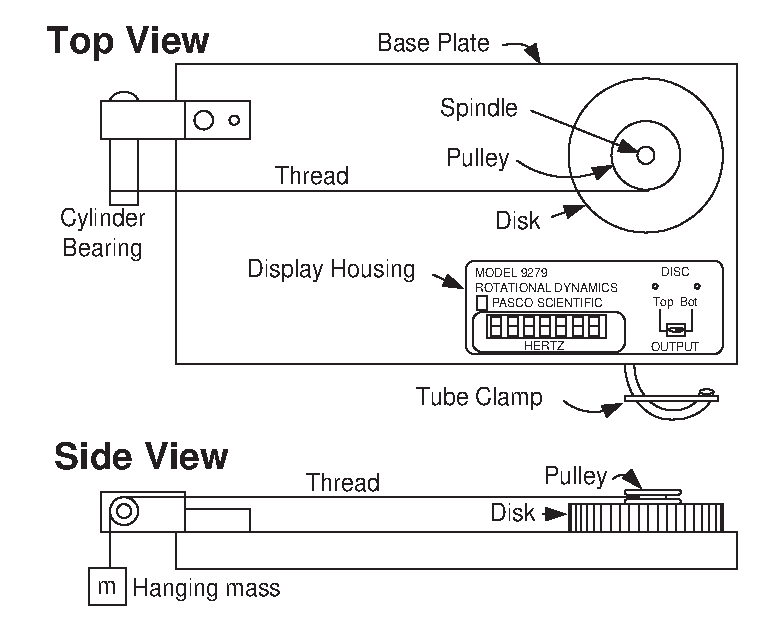
\includegraphics{Rotatefig.eps}}}}  %was diskB.eps
\end{center}
% \vskip.2in
% \vskip5.5in
% \special{bmp:disk.bmp y=5.5in}
 \caption{Rotational motion apparatus.  \label{fig:rot1}}
 \vskip.2in
\end{figure}

Consider the apparatus shown in Figures~\ref{fig:rot1} and
\ref{fig:rot2}.  We seek an expression for the rotational inertia
$I$ of the rotating system:  the rotating top disk with or without the object
(cylindrical ring or rectangular bar) placed on top of it.

First, we must find the torque that the string exerts on the top
disk.  The equation that relates torque to force is:
\begin{equation}
\vec{\tau} = \vec{r} \times \vec{F}
\end{equation}
where $\vec{F}$ is the force acting on the object, at a distance
$\vec{r}$ from
the axis of rotation.  Using the definition of the vector
product, we find that the magnitude of the torque can be written
\begin{equation}
\tau = rF \sin\theta
\end{equation}
where $\theta$ is the angle between $\vec{r}$ and $\vec{F}$.

As noted above, the torque is exerted by the
tension in a thread wrapped around a pulley.
Thus the force is the tension $T$ in the thread, and $r$ is the radius
of the pulley mounted on the top disk (see
Fig.~\ref{fig:freebody} and the right side of the side
view in  Fig.~\ref{fig:rot1}.)  Under these circumstances, the angle
$\theta$ will always be equal to $90^{\circ}$ making $\sin\theta = 1$.
Therefore, the torque on the system is
\begin{equation}
\tau = rT.
\end{equation}

To find an expression for the moment of inertia $I$ of the entire
system, we apply the rotational form of Newton's second law:
\begin{equation}
\tau = Tr = I \alpha.
\end{equation}
We also apply the linear form of Newton's second law to the
descending mass (choosing positive down):
\begin{equation}
mg -T = ma  \;\;\; {\rm or}
\end{equation}
\begin{equation}
mg -m \alpha r = T
\end{equation}
where we have used the usual relation between linear and angular acceleration,
$a=\alpha r$.  We combine these two equations to get the result
\begin{equation}
mgr = (I + mr^{2}) \alpha  .
\end{equation}
We could just solve this equation for $I$.  However, it will turn
out that the second term in the parentheses ($ mr^{2}$) is much smaller
than $I$. Consequently, to a very good approximation, we can neglect
this term.  If we do so, and solve for $I$, we obtain
\begin{equation}
I = {mgr \over \alpha}
\label{eq:rotfree}
\end{equation}


Equation E.10 then applies and 
the uncertainty in $I$ is given by
\begin{equation}
{\delta I \over I} = \sqrt{
                           \left( {\delta m \over m} \right)^2  +
                           \left( {\delta r \over r} \right)^2  +
                       \left( {{\delta \alpha} \over \alpha} \right)^2
                     }
\end{equation}
Be sure to include your derivation in your lab notebook.


\subsection*{Theoretical expressions for rotational inertia}

\paragraph*{cylindrical ring:}
The equation for the rotational inertia of a
cylindrical ring rotating about its axis is:
\begin{equation}
I = {{1} \over {2}} \, M \, \left( R_{\mbox{{\small out}}}^{2} +
    R_{\mbox{{\small in}}}^{2}
    \right)    \label{eq:rot2}
\end{equation}
where $M$ is the mass of the ring, $R_{\mbox{{\small out}}}$ is the
outer radius of
the cylinder, and $R_{\mbox{{\small in}}}$ is the inner radius.

The uncertainty is {\em approximately}:

%MathType!ZZhx47!eeaaduGcbmGdaaqacqizcGPasmysaeGedMeaaiGH9mqdaaqadeaaae
%WaoaaabiaHKjaMiiXGnbqasmytaaaacyjkcyzkamWdaaWcreGaikda
%aOGagUYabaaabiaIYmGdaaqacqizcGjcsmOud8qaaSqace4BceyDce
%iDaebaaOqasmOud8qaaSqace4BceyDceiDaebaaaaakiGLOiGLPaWa
%paaaleracGOmaaGccy4kdeaaaeGaikZaoaaabiaHKjaMiiXGsnWdba
%WcbiqGPjqGUbqeaaGcbiXGsnWdbaWcbiqGPjqGUbqeaaaaaOGawIIa
%wMcad8aaaSqebiaIYaaaaebaaaa!233A!
\begin{equation}
{{\delta \,I} \over I}=\sqrt {\left( {{{\delta \kern 1pt M} \over M}} \right)^2+\left( {2{{\delta \kern 1pt R_{out}} \over {R_{out}}}} \right)^2+\left( {2{{\delta \kern 1pt R_{in}} \over {R_{in}}}} \right)^2}
\end{equation}

\paragraph*{rectangular bar:}
The  equation for
the rotational inertia of a rectangular bar rotating about its center
of mass is: \begin{equation}
I = {{1} \over {12}} \, M \, \left( \ell^{2} + w^{2}  \right)
       \label{eq:rot3}
\end{equation}
where $M$ is the mass of the bar, $\ell$ is the length of the bar and $w$
is the width.

The uncertainty is {\em approximately}

%MathType!ZZhx47!eeaaduGcbmGdaaqacqizcGPasmysaeGedMeaaiGH9mqdaaqadeaaae
%WaoaaabiaHKjaMiiXGnbqasmytaaaacyjkcyzkamWdaaWcreGaikda
%aOGagUYabaaabiaIYmGdaaqacqizcGjccSiBaeGalYgaaaGawIIawM
%cad8aaaSqebiaIYaaakiGHRmqaaaqacGOmd4aaaeGaesMayIGedEha
%biXG3baaaiGLOiGLPaWapaaaleracGOmaaaaraaaaa!1944!
\begin{equation}
{{\delta \,I} \over I}=\sqrt {\left( {{{\delta \kern 1pt M} \over M}} \right)^2+\left( {2{{\delta \kern 1pt \ell } \over \ell }} \right)^2+\left( {2{{\delta \kern 1pt w} \over w}} \right)^2}
\end{equation}

%Be sure to include a derivation of the expression for the uncertainty
%in the theoretical value
%of whichever object you use, given the uncertainties in the measured
%quantities (mass and dimensions).   Use the methods developed in Appendix A.

\section*{Procedure}

%Before you begin, record in your lab notebook the masses and radii of the top
%and bottom steel disks. Label these quantities {\em clearly} so as not to
%confuse them with each other.  These quantities can be found on the base
%of the Rotational Dynamics unit.  Also record the radius of the pulley that
%you will use.  Measure its diameter using a caliper and divide this by two
%to get the radius.  You will need this quantity to calculate the applied torque.
%Also record the dimensions and mass of the square aluminum plate.

First check to make sure the unit is level by placing the bubble level
on the top steel disk.  The bubble should be centered in the level.
Then rotate the level $90^{\circ}$ and check the position of the
bubble again.  If it is not in the same position as before or is not
centered, the unit {\em may} need leveling --- ask your instructor to
examine your apparatus.  {\bf Note:} If the unit is not level, the
angular acceleration will not stay constant and your data may be
affected.

Once your unit is level, turn on the
air supply and adjust the regulator so that the air pressure is between 9 and 12 psi.
The air pressure is adjusted by turning the knob on top of the regulator.

Compressed air emerging from small nozzles in the base and
spindle form a cushion on which the top disk can float.  In
this way, friction is eliminated (or at least minimized).
The apparatus
uses an infrared detector to measure the passing of the light and dark bands on the
sides of the disk.  
%This quantity is shown in the display and has units of bands/sec or
%hertz (Hz).  
You can change which disk you are monitoring by toggling the
Top/Bottom switch.  
The wires emerging from the display box carry signals to
the computer so that the frequency of both the top and bottom disks can be
monitored simultaneously.  The Pasco software converts this signal
into angular velocity, so that one can measure the angular velocity of
the disk as a function of time.

On some units, there is a white tube clamp underneath the base of
the unit.  When it is closed, it allows the bottom disk to rotate freely on
the base.  When it is opened, the bottom disk will rest securely on the base.
Since we will only use the top disk in this part of the experiment, open the
tube clamp.  On other units this same function is controlled by a drop pin.

The top disk can be made to rotate freely on the bottom disk by plugging
the hole in the axle with a solid screw (or in Part II by filling
the hole with a drop pin)
%placing the drop pin or screwing a solid screw into the opening at the center
%of the disk.  
In this part of the experiment we will use the solid screw which must
thread the anchor washer (with attached string) and the pulley --- connecting both to the center of the top disk.
The anchor washer fits into the recess of
the pulley and the thread fits through the slot in the pulley.  The screw goes
through the hole in the square aluminum plate (if used, see Option A below), the pulley, the washer and into
the threaded hole in the top of the disk.  The thread comes out of the slot in
the pulley, runs over the groove in the cylinder bearing, and suspends the
falling mass.

In order for the mass supplying the torque to fall freely, place the apparatus
so that the cylinder bearing hangs over the edge of the table.
%Using the {\em solid, grey} screw secure the square aluminum plate
%(if needed---it is used only for the cylindrical ring), the thread
%anchor washer, and the small pulley to the hole in the center of the top disk.
\begin{figure}
\begin{center}
{\resizebox{4in}{!}{{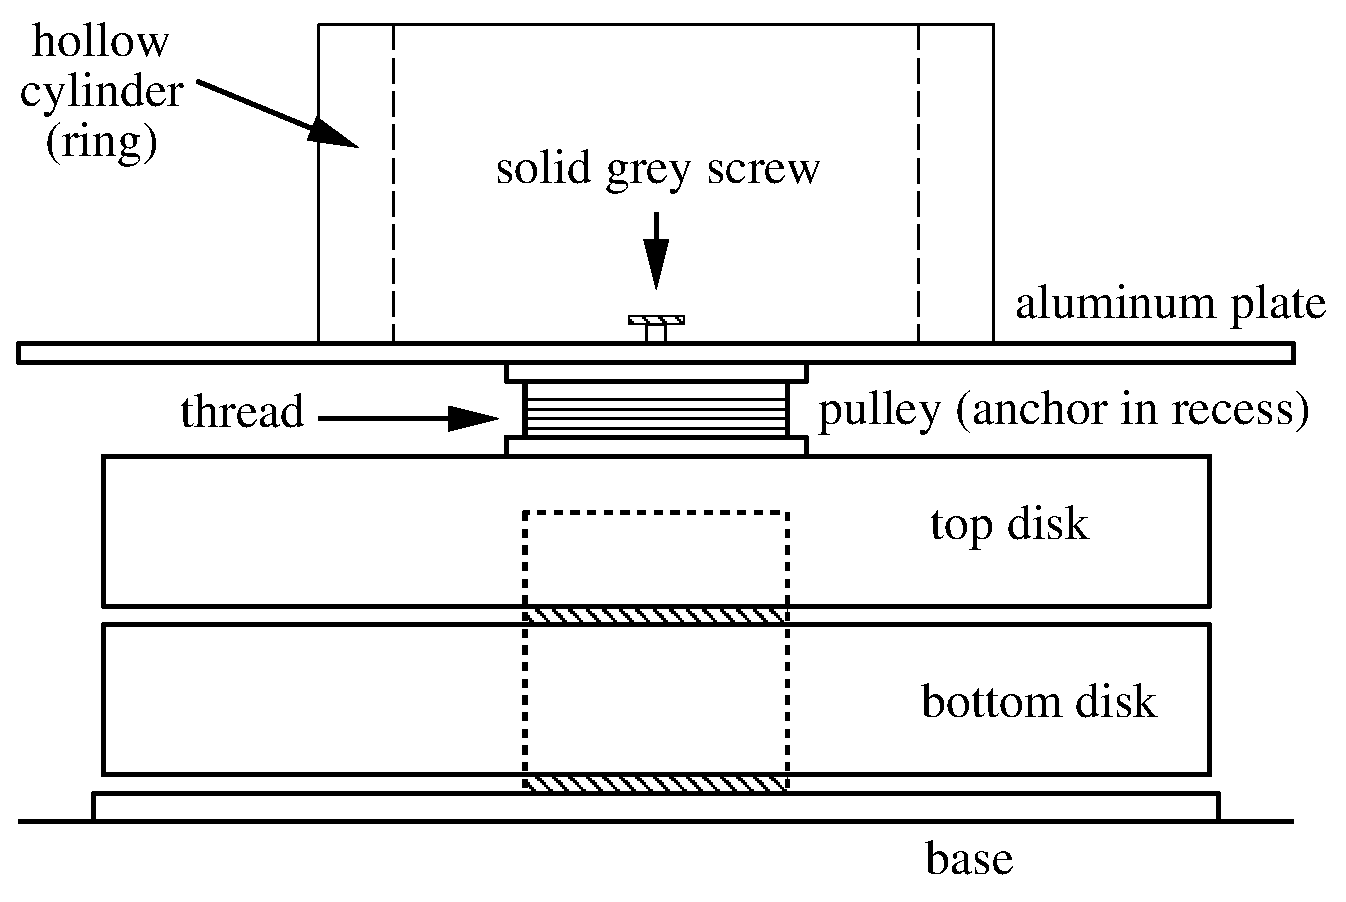
\includegraphics{plate.eps}}}}
\end{center}
%\vspace{2.75in}
%\special{bmp:plate.bmp x=5.5in y=2.75in}
\caption{Diagram for setting up the Moment of Inertia experiment.
  \label{fig:rot2}}
\end{figure}
See Figure~\ref{fig:rot2}.  

Now check to make sure that the air pressure is still at the right value for
your set-up (keep
monitoring the pressure throughout the experiment).  The bottom disk should be
stable (the tube clamp is open, or drop pin out) and the top disk should rotate freely.  By
{\em gently} turning the top disk, wind the thread around the pulley until the
top of the descending mass is level with the bottom of the cylinder
bearing
bracket.  Hold the top disk stationary for a moment and then release it, being
careful not to impart any initial angular velocity to the disk.  The falling
mass should accelerate the disk.  The thread should unwind from the pulley
and, before the mass hits the ground, the thread should begin to start winding
back on the pulley.  If the mass does hit the ground, shorten the length of
thread appropriately.  Make a couple of test runs to get used
to the equipment.  %Make sure the switch on the display housing is in the `TOP'
%position since only the top disk is rotating.

{\bf Note:  Observe a short ``mini" experiment on conservation of
energy at this point.}  After you drop the mass as outlined above, it
will reach its minimum point, and then rise again as the kinetic
energy of the disk is transferred back into the potential energy of
the small mass $m$.  See how near the mass gets to its original
starting position---very little energy is lost to friction in
this process.

%The next step is to get acquainted with the computer and software.
%You will be given a handout that describes, in detail, the steps to use
%the IBM PC and Pasco Interface for taking data.

%A couple of things to remember are:
%\begin{enumerate}
%\item Fifteen data points are sufficient.
%\item The number of dark bands per revolution is {\bf 200}.  Entering this value
%allows the program to convert the units from bands/sec to radians/sec.
%\item The number of dark bands per data point is {\bf 50}.  Entering this value
%tells the computer to measure the time it takes for 50 bands to pass the sensor.
%\end{enumerate}
%After entering the quantities enumerated above, the program will prompt you with
%\begin{verbatim}
%PREPARE TO RELEASE OBJECT
%PRESS ANY KEY TO CONTINUE
%\end{verbatim}
At this point wind up the thread and hold the disk steady.
Tell the Pasco
software to begin taking data, and then release top disk
plate {\em without imparting any initial angular velocity to it}.

%The computer will pause for a while for data taking and calculations.  When it
%is done with its calculations it will display information regarding the run on
%the screen.  {\em Copy down the value of the acceleration in your notebook}.
%You can view the displacement vs.\ time graph if you want, but {\em definitely}
%view the velocity vs.\ time graph.

Check the angular velocity vs.\ time graph to make
sure that it is a linearly increasing function of time. Continue until two
complete up-and-down cycles have been recorded and then hit Stop. Select a
linear portion of the data, and transfer it to \WAPP.  (Use $\delta \omega = .03$~rad/sec
and neglegible error in time.) Do a
least-squares fit to find the angular acceleration (the slope of the
graph of angular velocity vs. time).  You don't need to print the fit
report, but do be sure to record the angular acceleration in a data
table.

If your graph of angular velocity vs.\ time appears to be okay, continue to take three
more measurements of angular acceleration and record the absolute value of four values 
(two from up segments, two from down segments) in your
lab notebook in a data table.  When you analyze the data you will average the
four (now positive) angular accelerations and use the average acceleration to
calculate the moment of
inertia of the setup (i.e., the aluminum plate (if used), the pulley, and the
top disk).  The standard deviation of the mean\footnote{
Recall: see page \pageref{sdev.mean} or  \pageref{atwood.sdev.mean}.} will be the uncertainty
in the angular acceleration ($\delta\alpha$).

Our strategy will be to measure
the rotational inertia of the system with and without an object.  The
rotational inertia of the object alone will then be the difference
between these two values.  We have just measured the angular acceleration
without an object, so we must next:
%
\begin{itemize}
\item Measure the angular velocity as a function of time for
the system with the object.
%
\item Paste the angular velocity vs.\ time data into \WAPP, and do a
least-squares fit to find the angular acceleration.
%
\item Repeat the procedure outlined above, recording
four measurements of angular acceleration in a table. Calculate the
average angular acceleration and the standard deviation of the mean
($\delta \alpha$) just as you did before but now with the object aboard.
\end{itemize}

{\bf Select an object, add it to the system and measure the angular acceleration!}

\subsubsection*{Option A:  Rotational inertia of a cylindrical ring}
%Now you are ready to measure the moment of inertia of a cylindrical
%ring. 
Take either of
the two black, steel cylindrical rings and measure its mass and the
inner and outer diameters. Record these values in your
lab notebook.

The cylindrical ring is mounted on an aluminum plate, which will be
clamped to the top steel disk with the pulley between---your instructor will show you how.
Make sure to fit the locating pins on the ring into the holes
in the aluminum plate, so that the cylinder will rotate about its
center of mass.

\subsubsection*{Option B: Rotational Inertia of a Solid Rectangular
Bar} The procedure is similar to the one outlined above, except that
we will not need the aluminum plate.  First, record the
mass and dimensions of the rectangular steel bar in your lab notebook.

Secure the bar on top of the pulley (which is on top of the steel disk)
with the {\em solid, red}
screw.  The {\em red} screw will go through the bar, the pulley, the
thread
washer, and into the steel disk.

\section*{Data Reduction and Analysis}

For whichever object you used, you should have average angular
accelerations (with error) for the system with
and without the object.  To find the moment of inertia of the object
alone, proceed as follows:

\begin{enumerate}
%\item
%Collect your average accelerations in a table, along with their
%uncertainties.
%
%\item Find the torque exerted on the system by the descending mass,
%using the equations derived above.
%
\item Use Eq.~\ref{eq:rotfree} above to find the both rotational
inertias (with and without the object).
%
\item Find the uncertainty in both rotational inertias.
%
\item Subtract your experimental rotational inertias to find the rotational inertia of the object alone,
and calculate its uncertainty (see page \pageref{table1} or Appendix E).
%
\item Finally, calculate the theoretical value of the rotational
inertia, with uncertainty, and compare it with your experimental
result.
\end{enumerate}
Summarize your results in a carefully constructed table.

%Calculate the applied torque by multiplying the force ($F = mg$, where
%$m = 25\:$g and $g=980\:$g-cm/s$^{2}$) by the radius of the pulley.  This will
%give you the torque in units of g-cm$^{2}$/s$^{2}$.  When this torque is divided
%by the angular acceleration, you will get the moment of inertia in units of
%g-cm$^{2}$.
%
%Next find the average of the angular accelerations for your three sets of data
%(i.e., aluminum plate only, aluminum plate plus cylinder, and aluminum plate
%plus rectangular steel
%bar).  Also find the uncertainty in this average; the uncertainty will be the
%standard deviation of your five values.  Record these as
%$\bar{\alpha} \pm \sigma_{\alpha}$ where
%$\bar{\alpha} = \alpha_{\mbox{{\small average}}}$
%and $\sigma_{\alpha}$ is the standard deviation of your five values.
%
%Using your aluminum-plate-only data, calculate the moment of inertia of the
%aluminum plate plus top disk by dividing the torque by the average acceleration.
%Also record the uncertainty in this moment of inertia.  The moment of inertia of
%this system will be subtracted from the moments of inertia of the other two
%systems to find $I_{\mbox{{\small cyl}}}$ and $I_{\mbox{{\small bar}}}$.
%
%Using your aluminum plate plus cylinder data, find the moment of inertia of
%this system.  To get the moment of inertia of the cylinder only, subtract off
%the moment of inertia of the top disk/aluminum plate system.  Make sure you
%calculate the uncertainty associated with this value.  Also calculate
%the moment of inertia of the cylinder using mass amd dimension data and
%Eq.~\ref{eq:rot2}.  Compare these two values.  Are they in agreement?
%
%Using your aluminum plate plus rectangular steel bar data, find the moment of
%inertia of this system.  To get the moment of inertia of the bar only, subtract
%off the moment of inertia of the top disk/aluminum plate system.  Make sure you
%calculate the uncertainty associated with this value.  Also calculate
%the moment of inertia of the bar using mass and dimension data and
%Eq.~\ref{eq:rot3}.  Compare these two values.  Are they in agreement?

\begin{center}
{\Large {\bf Part II --- Conservation of Angular Momentum}}
\end{center}
\section*{Introduction}
Angular momentum, $\vec{L}$, can be written as the product of the moment of inertia,
$I$, and the angular velocity, $\vec{\omega}$. (Please see your
textbook for a more complete discussion.) In this experiment we will
see whether or not angular momentum is conserved.

The experiment works as follows:  We will set up the apparatus so that
{\em both} disks can rotate independently, and set them rotating at different
angular velocities, ${\omega}_1$ and ${\omega}_2$ (and thus with different
initial angular
momentum, ${L}_1$ and ${L}_2$).  Then, we collapse the air cushion between the two disks, so
that they come together and rotate {\em as a single body}, with some
final angular velocity ${\omega}_f$ and angular momentum ${L}_f$.  We can then
compare the initial and final angular momenta and see if
angular momentum is conserved:
\begin{eqnarray}
L_f &=& L_1+L_2 \label{eq:Lconserved1}\\
I_f \omega_f &=& I_1\omega_1+I_2\omega_2 \label{eq:Lconserved2}\\
{1\over2}M_f R^2 \omega_f &=& {1\over2}M_1 R^2\omega_1+{1\over2}M_2 R^2\omega_2 \label{eq:Lconserved3}\\
M_f  \omega_f &=& M_1 \omega_1+M_2 \omega_2 \label{eq:Lconserved4}
\end{eqnarray}
In this final form, conservation of angular momentum looks exactly like
conservation of linear momentum!

Remember that in such a `totally inelastic' collision, kinetic energy is not
conserved.  We can check by calculating the initial and
final kinetic energies.  %What would you expect, given the problems we
%have solved in class?

The computer will graph the angular velocities of the
two disks before, during and after the collision, allowing  you to select the initial and final
angular velocities.  %From these angular velocities you will calculate the
%initial and final angular momenta and kinetic energies.

\section*{Procedure}
Begin by closing the white tube clamp located underneath the base of the unit or
inserting the drop pin into the labeled valve.
Doing so will allow the bottom disk to rotate freely.

Record the masses %and radii 
of the top and bottom disks.%---these values will
%be supplied by your TA.  You will use
%them later to calculate the moments of inertia for the top and bottom disks.

Insert the ``drop pin'' in the hole in the top disk's axle, so that the top
disk will rotate independently of the bottom one.  (Your instructor
will show you how.) Spin the bottom disk fairly fast and the top disk
more slowly.  Spin the two disks in the {\em same direction}.  {\em
You must make sure that both disks have some initial angular
velocity}.

Tell the computer to start taking data.  Let it record the initial
angular velocities for several seconds, and then collapse the air
cushion by pulling the drop pin.  Stop the data collection a few
seconds after the collision when the disks are rotating as one.
%
%The Pasco DataStudio program will then display
Select from the resulting graph (a bit just before or after the collision)
the initial ($\omega_{1}$ and $\omega_{2}$) and final ($\omega_{f}$)
angular velocities. (If you select the $\Sigma$ button on the graph it
will display the mean $\omega$ for the data you select.)


%Run the experiment four times in all and collect you data in a table.
%Leave
%eight columns for the following quantities: initial angular momenta for the top
%and bottom disks, initial rotational kinetic energies for the top and bottom
%disks, final angular momentum for the two disks together, the final
%rotational kinetic energy for the two disks together, the change in angular
%momentum, and the change in rotational kinetic energy.

\section*{Analysis}
%---OUT---
\begin{comment}
First calculate the moments of inertia for the top and bottom disks using the
equation
\begin{equation}
I = {{1} \over {2}} \, MR^{2}.
\end{equation}
The moment of inertia for the combined top/bottom disk situation will just be
the sum of the individual moments of inertia.

Next start filling in the table mentioned above for each of the four runs.
The angular momentum is equal to
\begin{equation}
\vec{L} = I \vec{\omega}.
\end{equation}
If you spun both disks in the same direction as outlined above, you
can ignore the vector nature of this equation.  If you spun
the disks in opposite directions, the angular momentum of one disk
will be negative with respect to the other.  It doesn't matter which
one you call negative.

The rotational kinetic energy is equal to
\begin{equation}
K_{\mbox{{\small rot}}} = {{1} \over {2}} \, I \omega^{2}
\end{equation}

Next calculate change in angular momentum from the initial to the final state:
\begin{equation}
\Delta L = L_{1} + L_{2} - L_{3}
\end{equation}
where $L_{1}$ and $L_{2}$ are the initial angular momenta and $L_{3}$ is the
final angular momentum.  Record $\Delta L$ for the four runs in tabular form.
The percentage of angular momentum lost can be calculated from:
\begin{equation}
{{\Delta L} \over {L_{1} + L_{2}}}
\end{equation}
Also calculate the change in rotational kinetic energy:
\begin{equation}
\Delta K_{\mbox{{\small rot}}} = K_{1} + K_{2} - K_{3}
\end{equation}
where $K_{1}$ and $K_{2}$ are the initial rotational kinetic
energies and $K_{3}$ is the final rotational kinetic energy.  Record
$\Delta K_{\mbox{{\small rot}}}$ for the four runs in tabular form.
The percentage of energy lost can be calculated from:
\begin{equation}
{{\Delta K_{\mbox{{\small rot}}}} \over {K_{1} + K_{2}}}
\end{equation}
\end{comment}
%---END OUT---------
Conservation of angular momentum says the change in
angular momentum should be be zero:
\begin{equation}
\Delta L \equiv L_{f} -(L_{1} + L_{2})=0
\end{equation}
As shown above, because the disks have the same radius, this can be simplified to:
\begin{equation}
M_1 \omega_1+M_2 \omega_2 -M_f  \omega_f = 0\label{eq:Lconserved5}
\end{equation}
Of course, because of measurement uncertainty, it will not be exactly zero,
so the question becomes: is it consistent with zero when errors are considered?

Using Eq.~E.7 we find the error in a product $M\omega$ is given by:
\begin{equation}
\delta(M\omega)=\sqrt{(M\delta \omega)^2+(\omega\delta M)^2}
\end{equation}
Using Eq.~E.5 we find the error in the sum (or difference) of such terms in
Eq.~\ref{eq:Lconserved5} is given by:
\begin{equation}
\sqrt{\left(\delta(M_1 \omega_1)\right)^2+\left(\delta(M_2 \omega_2)\right)^2+\left(\delta(M_f \omega_f)\right)^2}
\end{equation}
which expands to
\begin{equation}
\sqrt{(M_1\delta \omega)^2+(\omega_1\delta M)^2+(M_2\delta \omega)^2+(\omega_2\delta M)^2+(M_f\delta \omega)^2+(\omega_f\delta M_f)^2}
\end{equation}

Use a spreadsheet to make this calculation easier! Note: for this process we estimate the
error in the measurement of angular velocity to be:
\begin{equation}
\delta\omega = 0.1\mbox{ rad/sec}
\end{equation}

\section*{Conclusions}
\subsection*{Part I}
Present the results obtained in Parts I of the experiment in a
carefully constructed table.  Be sure to include uncertainties and units.

Your discussion of the results should include (but is not limited to)
the following points:
\begin{itemize}
\item Comment on the agreement between the experimentally determined
and the
theoretical values for the moments of inertia in Part I.  Do they
agree within experimental uncertainty?  What are the sources of error?
%Are there any
%rotating bodies that we did not take into account?  If so, would they affect
%the outcome of the experiment significantly?
\item Were we quantitatively justified in neglecting the $mr^2$ term
when we derived Eq.~\ref{eq:rotfree}?  Do a quick calculation to
justify your answer.
\end{itemize}

\subsection*{Part II}
Present the results obtained in Part II of the experiment in a
carefully constructed table.
Comment on the extent to which angular momentum was conserved.
Angular momentum is  conserved only if there are no {\em
external}
torques acting on the system.  If your results show that the angular momentum
of the system was not conserved, could it be due to the presence of an
external torque or is it merely the effect of experimental
uncertainty?

%Was the rotational
%kinetic energy conserved?  Does this tell you that the collision was elastic
%or inelastic?

\section*{Critique}
Follow the suggestions in the Introduction to the Laboratory Manual.

\section*{Quick Report Card}
Properly report (sigfigs, units, error) your experimental value for the object's $I$.
Properly report (sigfigs, units, error) your theoretical value for the object's $I$.

From Part II, properly report (sigfigs, units, error) $\Delta L$, i.e., Eq.~\ref{eq:Lconserved5}.